\documentclass{tufte-handout}

%\geometry{showframe}% for debugging purposes -- displays the margins

\usepackage{amsmath}

% Set up the images/graphics package
\usepackage{graphicx}
\setkeys{Gin}{width=\linewidth,totalheight=\textheight,keepaspectratio}
\graphicspath{{graphics/}}

\title{Understanding Energy Balance}
\author{}
\date{}  % if the \date{} command is left out, the current date will be used

% The following package makes prettier tables.  We're all about the bling!
\usepackage{booktabs}

% The units package provides nice, non-stacked fractions and better spacing
% for units.
\usepackage{units}

% The fancyvrb package lets us customize the formatting of verbatim
% environments.  We use a slightly smaller font.
\usepackage{fancyvrb}
\fvset{fontsize=\normalsize}

% Small sections of multiple columns
\usepackage{multicol}

% Provides paragraphs of dummy text
\usepackage{lipsum}

% These commands are used to pretty-print LaTeX commands
\newcommand{\doccmd}[1]{\texttt{\textbackslash#1}}% command name -- adds backslash automatically
\newcommand{\docopt}[1]{\ensuremath{\langle}\textrm{\textit{#1}}\ensuremath{\rangle}}% optional command argument
\newcommand{\docarg}[1]{\textrm{\textit{#1}}}% (required) command argument
\newenvironment{docspec}{\begin{quote}\noindent}{\end{quote}}% command specification environment
\newcommand{\docenv}[1]{\textsf{#1}}% environment name
\newcommand{\docpkg}[1]{\texttt{#1}}% package name
\newcommand{\doccls}[1]{\texttt{#1}}% document class name
\newcommand{\docclsopt}[1]{\texttt{#1}}% document class option name

\begin{document}

\maketitle% this prints the handout title, author, and date

\begin{abstract}
\noindent This lecture will cover the basics of energy balance, including how we sense and measaure energy intake and expenditure.  This has very important consequences for understanding weight gain and loss, and understanding how different macronutrients are absorbed, stored and metabolized.
\end{abstract}

\tableofcontents

\pagebreak
\section{Learning Objectives}

\begin{itemize}
\item Apply the concept of energy balance to understanding weight gain and weight loss.
\item Explain the differences in energy content of various macronutrients.
\item Differentiate betwen the components of energy intake and energy expenditure and how evaluate how these contribute to energy balance.
\item Understand how energy balance and its various sub-components are changed in response to dieting.

\end{itemize}


\section{Energy Balance and Changes in Body Weight}

Obesity is now a major problem in most societies, with recent estimates showing that in America 38\% of adults\cite{Flegal2016} and 17\% of children \cite{Ogden2016} considered obese.  Fundamentaly, people gain weight because of altered energy balance.  This means that if energy intake is larger than energy expenditure, weight (primarily in the form of stored fat) will increase.  This unit will give an overview as to how we define and talk about energy balance.

\newthought{It may seem a bit abstract} to think of food, exercise and body weight all in terms of energy, but fundamentally every molecule of our body has a different caloric content, and when it is oxidized that energy is released.  In fact, ultimately all metabolic processes end up generating some heat, and the production of this heat, known as thermogenesis is an important part of understanding energy balance.  We all have intuitive ideas about someone's metabolic rate whether it be how one person can eat a large meal, while another seems to restrict their diet but is unable to lose weight.  Here we will discuss some of the physiology that makes up that energy balance and how this is modified by changes in diet.

\section{Energy Intake}

\subsection{What is Energy Intake?}
Energy intake is the sum of the amount of energy that is taken up by a person.  While a major part of this is the amount of food we eat, a less appreciated aspect is the efficiency of nutrient extraction during digestion.  As Dr. Anderson has covered in her introduction to digestion, food passes through our bodies and efficient digestion involves extracting as many nutrients as possible from the bolus of food.  Therefore we can consider energy intake as:

\begin{equation}
Energy_{intake} = Energy_{ingested} - Energy_{excreted}
\end{equation}

This is important to keep in mind, because different foods have both different energy content and different aptitudes towards being absorbed by the body.

\subsection{How do the foods we eat affect in energy intake?}

\begin{margintable}
\centering
\caption{Caloric density of the three major macronutrients and ethanol.  These values are known as Atwater's rules}
\label{tab:atwater-values}
\begin{tabular}{cc}
\hline
\textbf{Macronutrient}       & \textbf{Energy Density}                     \\
\hline
Carbohydrates & 4 kcal/g \\
Proteins & 4 kcal/g \\
Lipids & 9 kcal/g \\
Ethanol & 7 kcal/g \\
Fiber & 2 kcal/g \\

\hline
\end{tabular}
\end{margintable}

In general, since we know how much energy is contained per gram of each of the major macronutrients (see Table \ref{tab:atwater-values}).  These amounts, were calculated by Atwater and colleagues in the early twentieth century from determining how much heat was produced by burning pure fat, protein or carbohydrates\sidenote{Generally oxygen consumed is calculated rather than heat generated, a method known as indirect calorimetry}.  These values are listed in the nutritional information for many foods, and you might expect that the caloric density of your meal may be calculated by performing indirect calorimetry experiments on these foods.  This is not the case, in general food manufacturers use the composition of their food (in terms of macronutrients) and Atwater's rules to calculate energy density.  This can be misleading, since it refers to the complete energy content of a fuel and not necessarily the amount of calories actually absorbed by a typical person.

\subsection{How do we assess energy intake?}

The ideal way to assess energy intake might be to determine the caloric content of all the foods eaten by a person, for example by indirect calorimetry of an identical meal and then subtract the energy remaining in feces.  The FDA suggests that a normal health woman eats 2000 kcal per day (2500 for men).  To actually assess $E_{ingested}$ we generally make use of dietary recall surveys, and then compare the amounts and types of foods to a reference database.  A commonly used Food Frequency Questionaire can be found here: \url{http://bit.ly/2oucJw8}.  There is substantial debate in the research community regarding the accuracy and biases of the different types of dietary recall assessments\sidenote{These techniques will be covered in much more detail in \textbf{NUTR640: Nutritional Assessment}}.


\section{Energy Expenditure and Adaptive Thermogenesis}

The other side of the energy balance coin is energy expenditure, how how calories are used.  While energy intake is difficult to measure, energy expenditure is even harder to measure accurately without specialized equipment.  
\subsection{What are the components of energy expenditure?}
Energy expenditure can be broken down into several components which add up to one's total daily energy expenditure (TDEE).  This is shown schematically in Figure \ref{fig:tdee-components} taken from a review on the topic\cite{Tam2015}.  These include the basal metabolic rate (BMR), diet-induced thermogenesis (DIT), non-exercise activity thermogenesis (NEAT) and exercise activity thermogenesis (EAT)

\begin{equation}
TDEE = BMR + DIT + NEAT + EAT
\end{equation}

\begin{figure}
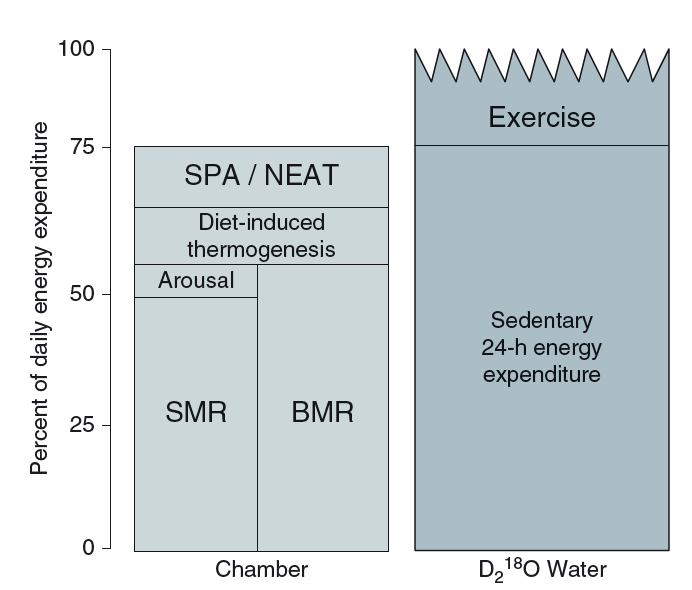
\includegraphics{figures/tdee-components.png}\
\caption{Components of total daily energy expenditure.  SMR represents sleeping metabolic rate.}
\label{fig:tdee-components}
\end{figure}

Each of these components have many complex factors that affect their magnitude, including genetics diet activity levels and others.  What should be apparent from Figure \ref{fig:tdee-components}, is that contrary to many people's intuition, exercise generally comprises only a small portion of total energy expenditure.

\subsection{How do we calculate energy expenditure}

The major factors that contribute to non-EAT energy expenditure are age (declines with age), sex (approximately 11\% higher in males) and body mass, particularly fat-free (or lean) mass.  Up to 85\% of the variance in BMR can be explained by these factors, with a further 11\% being heritible \cite{Bogardus1986}.   While we can approximate a person's TDEE based on gender, age, sex, and body composition this tends to be fairly inaccurate.  There are two main ways in which energy expenditure can be experimentally determined.

\newthought{Indirect calorimetry} monitors oxygen consumption and carbon dioxide production, typically over several hours or days.  This can be done in large rooms called metabolic chambers where an individual can live for several days.  The amount of oxygen consumed along with the amount of carbon dioxide produced can be converted into a measure of energy used, in the same way that food combustion can be used to determine the energy content of a meal.  This approach has several advantages, including the fact that DIT, EAT and NEAT can separately be calculated based on whether the individual is currently eating, moving etc.  The major disadvantage is that the subject has to remain in the room to be monitored.

\newthought{Doubly labelled-water} on the other hand allows the subject to go home and live their normal life, which might be a better approximation of their natural energy expenditure rates.  This technique is based on the differential release of isotopes after a subject drinks radiolabelled water ($^2H_2^{18}O$).  The hydrogen atoms are released only with water, but the oxygen atoms are released as CO$_2$ and water.  Because of the slower equillibration process it does not provide the temporal resolution of indirect calorimetry, but rather provides an integrated measure of total CO$_2$ production ovr the time peroid.

\subsection{How does diet affect energy expenditure?} 

\newthought{Diet-induced thermogenesis}, also known as the thermic effect of food represents the energy that is used in digestion, absorption and storage of food.  While it only accounts for 5-15\% of TDEE it is the most affected by nutrition choices.  Both meal size (larger, less frequent meals have higher TEF) and macronutrient composition (protein exerts a higher DIT) are major factors in DIT, along with genetics, age, activity levels and insulin sensitivity.  This is true for the short-term effects of specific meals, but over a longer term, changes in body composition also affects total energy expenditure.

While it was once thought that lower TDEE could be causal of obesity, careful studies in the early 1990s showed that obesity was associated with \emph{higher} energy expenditure rather than lower energy expenditure\cite{Ravussin1982}.  This is now thought to be an adaptive response to gaining weight.  When excess calories are consumed, the body responds by increasing the metabolic rate to try to maintain homeostasis.  Supporting that, during weight loss, the metabolic rate actually \emph{decreases}, likely again in an attempt to avoid changes in body weight\cite{Leibel1995a}.  Unfortunately for those trying to stay at a lower weight, this persistent reduction in metabolic rate lasts for many years \cite{Rosenbaum2008}.  Further complicating efforts in weight reduction, studies that have assessed appetite and appetite-driving hormones in successful dieter have shown that there are chronic feelings of both hunger and hunger hormones, again many years after weight loss \cite{Sumithran2011}.  These two factors, reduced TDEE and increased drive towards Energy Intake are major reasons why successful weight loss is so difficult.


\bibliography{library}
\bibliographystyle{plainnat}

\end{document}
